\documentclass[../memory.tex]{subfiles}

\begin{document}
\chapter{Introduction}
\section{Project introduction}
\emph{Recurrent travel} is a master's thesis for the Architecture and Design of
Software of the La Salle URL university.
\\
The project is being developed in the context of the increasing demand for air
transportation and the digitalization of the travel industry. This project aims
to offer an innovative solution for those users who frequently travel for work
or personal reasons, through the creation of an application that allows them to
be notified of opportunities on their regular routes.
\\[8pt]
This masters's thesis is framed in the ambit of project planning and management,
software design and clean software architectures, databases, testing, user
interface design and user experience.
\section{Project structure}
Even though the project was a team effort, this thesis will primarily focus on
the frontend development of the project. I have actively worked on and been
involved in the decisions regarding the frontend application development.
\\[8pt]
However, the thesis will also cover certain aspects of the backend, including
key concepts, a brief explanation of its architecture, and how the frontend
utilizes the API.
\section{Context}
Throughout the past decades, the European air transportation sector has
undergone an unprecedented growth, primarily propelled by the democratization of
pricing and the digitization of airlines. This expansion has resulted in a
noticeable increase in the number of users who utilize both domestic and
international flights.
\\[8pt]
In 2019, the volume of work flights increased to 1.28 billion
dollars\cite{flight-volume} and, even with the COVID-19 pandemic, the volume
kept going up\cite{covid-flight-volume}. Business trips are essential for both
interpersonal connection development and building trust between different
companies\cite{company-trust}. Business trips are often conducted to visit
the client, with over 44\% of the business trips in Europe being made for
client meetings and 32\% for visiting the company offices in other
cities\cite{visit-client}. Moreover, 30\% of business travelers in Europe travel
once a month, 62\% once a year, and 5\% between 21 and 40 times a
year\cite{visit-client}.
\\[8pt]
Group business trips are also a commonality, with over 50\% of such being made
by two or more workers\cite{visit-client}. When choosing a flight, 26\% of the
travelers in Europe will consider direct connections as the most important
aspect of a flight, 19\% will consider the price of the flight, 23\% schedule
coordination, and airport location 20\%\cite{visit-client}.
\\[8pt]
Taking into account the data before the COVID-19 pandemic, it is starting to be
more common that employees are responsible of the booking of their own travels,
with up to a 59\% of them travelling in the United States, being also
responsible to book the hotel\cite{employee-books}. Around the 69\% of the
travelers states that they book all the reservations, regardless of the type.
Additionally, 79\% of the business traveler have booked a trip through their
mobile devices, indicating the increased use of mobile technology for this
purpose\cite{mobile-booking}.
\\[8pt]
In the post-pandemic work (2023), commercial aviation continues to be efficient,
resilient and a key component to the development of the modern world. According
to the annual report by IATA\cite{iata-report}, it is expected that by the end
of 2023, all regions will have surpassed pre-pandemic flight demand.
Additionally, the charts how an average positive variation of 5.4\% points in
real GDP in the coming years.
\begin{enumerate}[label = -]
	\item For 2023, it is projected that the number of passengers will exceed
	      pre-COVID-19 levels, reaching up to 105\%.
	\item By 2030, it is estimated that the number of global passengers will grow
	      to 5.6 billion.
\end{enumerate}
Consequently, medium-term growth forecasts for commercial aviation indicate a
promising and expansive future for the sector.
\begin{figure}[H]
	\centering
	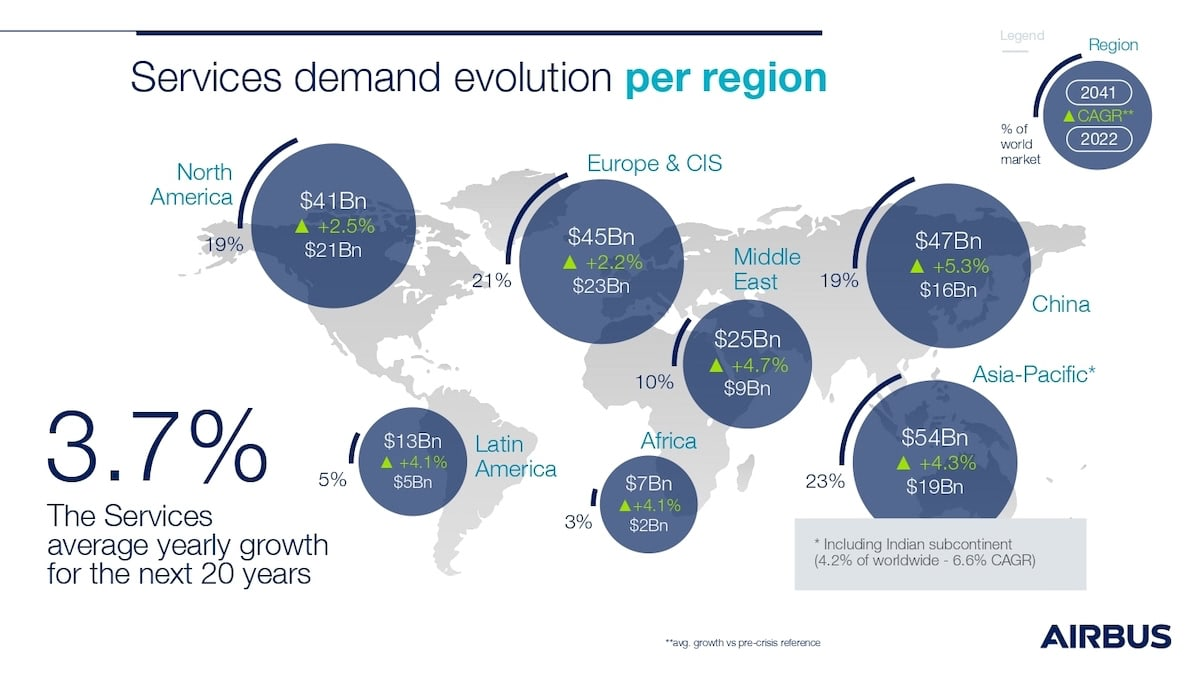
\includegraphics[width=\textwidth]{./assets/airbus-service-demand.png}
	\caption{Evolution of flight demand of Airbus flights in the pre-pandemic
		world vs the post-pandemic.}
\end{figure}
Within this context of growth, it has appeared another type of user: recurrent
travelers. This travelers, whether due to work, family or personal reasons,
have incorporated the use of planes into their routine periodically throughout
the year.
\\[8pt]
Recurrent trips are characterized by sharing the same point of origin and
destination, similar departure and arrival times on all routes, and a stable
repetition frequency throughout the year. Although airline digitalization and
the ease of purchasing plane tickets online have greatly simplified the process,
recurrent travelers still face difficulties when it comes to finding
opportunities and optimizing their itineraries. The lack of specific solutions
for this group of users has generated a growing demand for an application that
notifies them of opportunities on their recurrent trips, facilitating the
planning and management of their habitual travels.
\\[8pt]
Given the importance and frequency of business travel and the growing trend of
employees taking care of their own reservations, it is crucial to address the
callenges faced by these recurrent travelers.
\section{Solution proposal}
Throughout the project, we will focus on critical topis in software engineering.
The hexagonal architecture will be addressed due to its ability to facilitat the
development maintenance, and modification of software by separating
responsibilities into logical layers, thus promoting efficient code maintenance
for the product.
\\[8pt]
Domain-Drive Design (DDD) is an architecture pattern that emphasizes in solving
specific business problems, improving communication and the efficiency of the
software model. Applying DDD will help us create software that is more
understandable and effective by focusing on the different domain concepts of
Recurrent Travel.
\\[8pt]
Additionaly, the SOLID principles will be used ofr designing a modular,
understandable, and extensible software. These principles are essential for
establishing quality and maintainability standards in software component design.
It also ensures the creation of a robust, reliable, and easily maintainable
solution.
\\[8pt]
To ensure reliability and proper functioning of our application, testing and
validation techniques will be implemented.. Continuous Integration (CI) and
Continuous Development (CD) will also be taken into account as part of the
development cylce. Automation and version deployment will also take a spot in
the cycle.
\\[8pt]
Furthere, the integration with external systems will also be studied. This can
improve the efficiency of our software solution by leveraging the functionality
of other existing services in the market.
\\[8pt]
Finally, the importance of good practices in software development will be
strongly emphasized, focusing on resource management, risk mitigation, effective
communication, and develivering an mvp that meets customer expectations.
\\
Ultimately, this master's thesis project aims to offer an effective and
efficient solution to enhance the experience of recurrent travelers, enabling
them to optimize their trips and facilitate the planning and management of their
regular travels.
\section{Topics and concepts}
Before moving into the details of the project, it is fundamental to be
familiarised with some key concepts regarding software architecture and design,
which will be addressed throughout this projet. In this regard, we will
distinguish between general concepts, independent of the technology and
environment inwhich they will applied, and more specific concepts for the
backend and frontend development.
\subsection{General concepts}
Before starting, it has to be taken into account the concepts about software
architecture and design in the different applications to develop. As explained
in the goals of the project, the software to be developed should be scalable,
mantainable and robust.
\\[8pt]
In first place, it is essencial to consider the meaning of software desing.
Software design refers to the creation of a logical and organised structure
taking into account from the architecture, to modularity, reusability and
readability of the code.
\\[8pt]
Therefore, as a team we opted to apply hexagonal architecture as the foundation
of our applications. Hexagonal architecture is a software pattern whose goal is
to separate between business logic of its technical concerns. In order words, it
separates the domain of an application from the logic it may have. It also
promotes a greater independence between the components and simplifies the
adaptation to underlying technological changes. Additionally, it promotes
modularity and code reusability. The clear separation of responsibilities of
each layer and component, it facilitates the maintenance and evolution of
applications over time. Another important aspect about hexagonal architecture is
its focus on interfaces and contracts. The definition of such interfaces and
contracts ensures a more efficient communication and facilitattes the
integration with other services or external systems.
\\
Alongside hexagonal architecture, the team has opted to apply domain driven
design in our projects. DDD is a methodology that it is focused in modeling the
core business, focusing in specific concepts and rules of the domain. In this
project, DDD allows to precisely define entities, value objects and aggregates
from the current domain. Furthermore, the domain driven design allows the team
to establish a common language between the members of the team, providing a more
effective communication and a shared knowledge of functionalities and
requirements.
\\
It is also important to note the well-known SOLID principles, which have been
used to develop a better software, at a lower level than the aforementioned
concepts. Although not strictly an architectural concept, SOLID principles are
equally imporant in terms of development, as they promote code modularity,
extensibility and maintainability.
\\[8pt]
Regarding the deployment of the applications that will conform the system, the
team has opted for cloud solutions. The usage of a cloud environment offers a
set of significant advantagws in terms of scalability, availability and
flexibility, which are properties that are wanted for the project.
\\
The cloud, also known as \emph{cloud computing}, refers to the management of the
infrastructure and computing services over the internet, instead of hosting the
applications in local servers.
\\
Furthermore, deploying the applications in the cloud frees the team from
maintaining the underlying infrastructure. The cloud service provided will take
care of the server management, networking, and other required resources,
allowing the team to focus on the development.
\\[8pt]
Once the architecture and deployment aspects have been explained, it is crucial
to incorporate an element that strengthens the robustness of the system:
testing. In this project, two types of tests are distinguised: unit tests and
functional or acceptance tests. It is worth mentioning that testing is not
limited to this two types, many more types of testing exist, but such will not
be covered in this specific project.
\\
On the one hand, unit testing aims to validate the correct functioning of
individual units or functional pieces of code. While the main objective is to
ensure the expected functioning of such elements, their true value emerges in
the future when modifications need to be made to old or legacy code. When making
changes to existing code, developers may not take into account all the potential
side effects that may arise from such changes. Thus, unit testing provides
validation and security to the developer, ensuring that their changes do not
break any existing functionality.
\\
On the other hand, it is also essential to include functional tests alongside
unit test. These tests aim to validate the overall behaviour of a system by
attempting to recreate as close as possible the production environment. The
focus relies on component interaction and complete workflows or user flows.
Functional tests are particularly useful for detecting potential issues in the
integration of different modules or components of the system. By simulating the
real usage, it becomes easier to identify problems in communication between
components, errors in business logic, or differences in user experience.
\\
The combination of both type of tests, unit and functional, provides a
comprehensive testing approach that covers both the internal validation of each
component and the overall verification of the system as a whole.
\subsection{Backend concepts}
The backend for the Recurrent travel appliction is the core of data processing
in order to simplify the user experience in terms of finding travels. This
application layer it is crucial for its functionality and system performance.
However, it is not direclty exposed to the client, meaning that it will require
of a frontend.
\\
When developing the frontend, it is really important to keep scalability and
performance as the two main factors of the applications.
\subsubsection{Gradle}
Gradle is an advanced and flexible build automation system. Unlike other
systems, it uses a Groovy-based language for its configuration file, which is
more readable and easier to understand.
\begin{enumerate}[label = -]
	\item Dependency Management: It allows for efficient and flexible dependency
	      management, which is vital in a project of this scale.
	\item Automation: It is used to automate the build and deployment process,
	      making updates easier and ensuring that all parts of the system are
	      synchronized.
	\item Versatility: It supports both Java-based projects and other languages
	      like Kotlin, making it extremely flexible for any language change or future
	      additions. This ensures that this project has the freedom to adapt and
	      evolve over time.
	\item Performance: It is designed to perform well in large-scale projects,
	      thanks to features like caching and incremental execution. This means that
	      only the parts of the project that have changed since the last build will be
	      compiled, saving time and resources. This is especially valuable for this
	      project, which can grow in complexity over time.
	\item Integration with IDEs and CI/CD: It integrates well with popular
	      integrated development environments (IDEs) like IntelliJ IDEA and Eclipse.
	      This means that developers can use and manage Gradle directly from their IDE.
	      It also integrates with continuous integration/delivery (CI/CD) tools like
	      Jenkins and Travis CI, facilitating automatic deployment and updates.
\end{enumerate}
Therefore, the choice of Gradle for Recurrent travel not only facilitates
dependency management and project automation but also provides a solid and
flexible foundation for the project's evolution and growth in the future.
\subsubsection{Java}
Java is a widely used programming language known for its portability,
efficiency, and support for object-oriented programming.
\begin{enumerate}[label = -]
	\item Portability: Java is platform-independent, allowing the backend code to
	      run on any operating system that has the Java Runtime Environment (JRE)
	      installed, facilitating deployment and scalability.
	\item Maturity and Community Support: It has been a staple in the software
	      industry for over two decades, which means it has a wealth of libraries,
	      frameworks, and community support.
	\item Reliability and Stability: Java has a long track record of reliability
	      and stability, making it a safe choice for critical and large-scale
	      applications. Its strong exception handling system and automatic garbage
	      collector help minimize errors and prevent memory leaks, improving overall
	      application robustness.
	\item Security: Java was designed with security in mind. Its security features
	      include a strong type system, bytecode verification before execution, and
	      absence of pointers, helping prevent common errors that can lead to security
	      vulnerabilities.
	\item Support for Enterprise Development: It provides a rich ecosystem of
	      frameworks and libraries for enterprise development, such as Spring,
	      Hibernate, and Apache Camel, among others. These tools simplify the
	      implementation of a variety of backend functionalities, from database access
	      and security to integration with other systems and services.
\end{enumerate}
Therefore, choosing Java as the programming language for the backend of
Recurrent travel provides a solid and robust foundation for building a secure,
scalable, and high-performance application.
\subsubsection{Spring boot}
Spring Boot is a framework that simplifies the configuration and deployment of
Spring-based applications.
\begin{enumerate}[label = -]
	\item Rapid Development: It provides default configuration that accelerates
	      development by eliminating the need for extensive manual configuration.
	\item Integration: It integrates with many tools and libraries, such as
	      Hibernate for data persistence and Spring Security for security, making it
	      easy to implement these features.
	\item Integration with DevOps: It integrates well with DevOps practices and
	      tools. For example, it integrates with Jenkins for continuous integration
	      and with Docker for containerization, facilitating development, testing, and
	      deployment of applications.
\end{enumerate}
In summary, choosing Spring Boot for the development of this project enables
quick startup, scalability, and easy maintenance. Its wide range of features and
integrations facilitate the creation of a high-quality application that meets
the demands and expectations of frequent travelers.
\subsubsection{Unit test}
The implementation of testing is a crucial component to ensure software quality
and user satisfaction in this project. In the context of unit testing,
technologies like JUnit and Mockito are used.
\\[8pt]
JUnit is the most widely used unit testing framework for Java that helps
developers design and execute tests to verify the behavior of small units of
code, such as individual methods or classes. In this project, the usage of JUnit
provides the following benefits:
\begin{enumerate}[label = -]
	\item Quality Assurance of Code: By using JUnit for unit testing, it can be
	      ensured that each unit of code functions correctly before integration. This
	      helps detect and correct errors early in the development cycle.
	\item Facilitates Updates and Maintenance: Unit tests with JUnit facilitate
	      updates and maintenance of the application. Whenever a change is made to the
	      code, unit tests can be executed to ensure that the changes haven't
	      introduced new errors.
\end{enumerate}
Mockito is a popular Java mocking framework used to mimic objects and
behaviors of the test class. For the project, Mockito can be used to
simulate application logic that is not directly related to the code unit
being tested, such as database dependencies. The benefits of Mockito in this
context include:
\begin{enumerate}[label = -]
	\item Isolation of Code Units for Testing: It allows creating simulated
	      objects (mocks) of external dependencies, meaning that unit tests can focus
	      on the code under test without worrying about the behavior of dependencies.
	      This makes the tests more reliable and easier to write.
	\item Simulation of Diverse Test Scenarios: It is possible to simulate a
	      variety of test scenarios, such as the behavior of the application when an
	      external service fails or returns unexpected data. This helps ensure that
	      Recurrent travel can properly handle these situations in production.
\end{enumerate}
In summary, the combination of JUnit and Mockito enables comprehensive and
effective unit testing in "Recurrent Travel," resulting in more reliable and
maintainable software.
\subsection{Frontend concepts}
In terms of frontend development, it is important to consider the same concepts
mentioned in the first section. Although more details will be covered in future
sections, unlike server repositories, the client repository has been developed
as a mono-repository. There is a difference between a mono-repository and a
multi-repository, such as:
\begin{enumerate}[label = -]
	\item\emph{Multirepo}. The multirepo approach means to have multiple
	applications in different repositories. The main benefits of such approach
	are the fact that teams can separately work in the repository while at the
	same time the repository is kept smaller and cleaner.
	\item\emph{Monorepo}. The monorepo approach is the opposite of the multirepo:
	all the applications are developed from the same repository. Such approach
	allows maintaining build and deployment patterns altogether. However,
	application versioning may be harder to manage.
\end{enumerate}
When aiming to develop a client-scalable application while maintaining a single
shared domain layer, the mono-repository architecture has been preferred.
\subsubsection{Nx}
One of the main challenges that a team can face when working with a
mono-repository is its maintenance. Maintenance includes tasks such as library
updates and managing CI/CD pipelines, if they exist.
\\
Fortunately, there are tools that simplify this maintenance, known as build
tools. In the JavaScript world, a tool called Nx has gained significant
popularity. Translated from its documentation: \emph{Nx is a next-generation build
	system with first-class support for mono-repositories and powerful
	integrations.}\cite{nx}
\\[8pt]
The use of such a tool significantly simplifies the maintenance of JavaScript
and/or TypeScript mono-repositories. Some of its other strong points are:
\begin{enumerate}
	\item The same developers of Nx maintain plugins and similar tools that are
	      easily integrated with an existing repository.
	\item Instant generation of internal libraries.
	\item The ability to run tests and deployments only on the affected parts,
	      that is, on the modified code, allows limiting the necessary work in
	      Continuous Integration (CI) environments. This involves running tests for
	      the modified code and its dependencies.
	\item All created libraries and applications include all the necessary
	      dependencies, scripts, and tools for serving, testing, building, and
	      deploying in a streamlined manner.
	\item It provides a rich ecosystem of plugins and utilities within the same
	      base library.
\end{enumerate}
Furthermore, it provides extensive support for the most commonly used libraries
and frameworks in frontend development, such as NextJs, the chosen library for
developing the frontend application.
\begin{figure}[H]
	\centering
	
\includegraphics[width=0.2\textwidth]{./assets/logos/nx-logo.png}
	\caption{Nx logo}
\end{figure}
\subsubsection{TypeScript and JavaScript}
Currently, JavaScript is the most widely used language worldwide for many
reasons. However, due to its lack of types, some applications become harder to
debug and more error-prone. That's one of the reasons why Microsoft developed
TypeScript, which is a strict syntactical superset of JavaScript. Code written
in TypeScript is transcompiled to JavaScript during the build time.
\\
By using TypeScript, we provide a highly productive environment when developing
the different applications. It not only reduces the number of hard-to-detect
errors caused by type issues but also provides all the benefits of ECMAScript.
\begin{figure}[H]
	\centering
	
\includegraphics[width=0.175\textwidth]{./assets/logos/js-logo.png}
	
\includegraphics[width=0.175\textwidth]{./assets/logos/ts-logo.png}
	\caption{JavaScript and TypeScript logos}
\end{figure}
\subsubsection{NextJs}
As mentioned before, Next.js has been chosen as the front-end framework to build
the applications with. This framework is built on top of Node.js, which enables
React-based web application functionalities such as server-side rendering (SSR)
and static websites. On the Next.js homepage, they provide the following
description: \emph{Used by some of the world's largest companies, Next.js
	enables you to create full-stack Web applications by extending the latest React
	features, and integrating powerful Rust-based JavaScript tooling for the fastest
	builds}\cite{nextjs}.
\\[8pt]
Development with Next.js involves structuring the code in a specific way so
that the compiler can generate packages in the most efficient manner,
avoiding unnecessary code being sent to the client and thus reducing page
load time. This feature is known as code-splitting.
\\
React is a framework designed to simplify the construction of web components. As
it gained popularity, developers started building full-fledged applications
based on React. However, this meant serving a large amount of JS code to the
client, which slowed down webpage loading. Next.js automatically solves this
problem without the need for any configuration.
\begin{figure}[H]
	\centering
	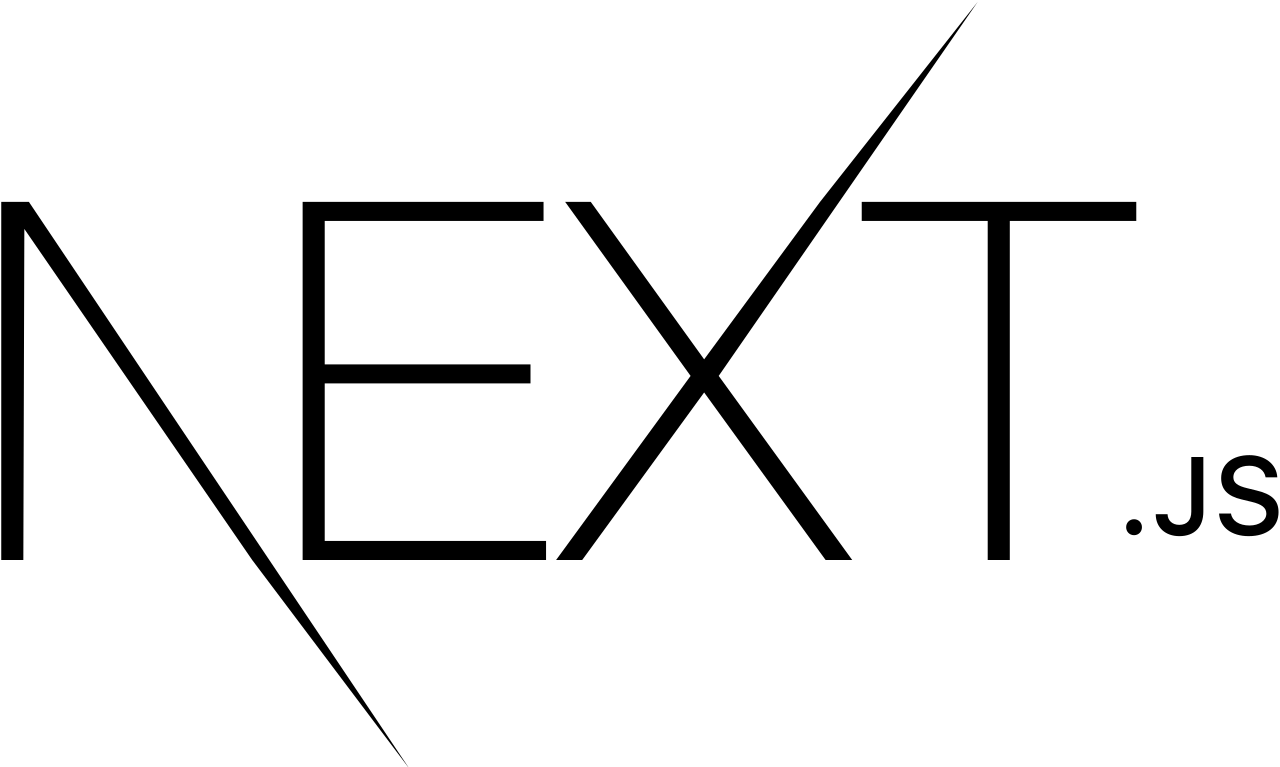
\includegraphics[width=0.2\textwidth]{./assets/logos/next-logo.png}
	\caption{Next logo}
\end{figure}
Development with Next.js involves structuring the code in a specific way so that
the compiler can generate packages in the most efficient manner, avoiding
unnecessary code being sent to the client and thus reducing page load time. This
feature is known as code-splitting.
\\
React is a framework designed to simplify the construction of web components. As
it gained popularity, developers started building full-fledged applications
based on React. However, this meant serving a large amount of JS code to the
client, which slowed down webpage loading. Next.js automatically solves this
problem without the need for any configuration.
\subsection{Unit and acceptance testing}
The importance of testing has already been mentioned, and the client is no
exception. Testing the client brings the same benefits as testing the server, as
it is the part that will be used by the end user. Nx provides plugins to enable
testing with different libraries.
\begin{figure}[H]
	\centering
	
\includegraphics[width=0.2\textwidth]{./assets/logos/jest-logo.png}
	\caption{Jest logo}
\end{figure}
At the unit testing level, both for the domain code and the component code, the
Jest library has been used. Jest is a unit testing and mocking library developed
and maintained by Facebook. Currently, it is one of the most famous, if not the
most famous, libraries for testing. It provides a powerful CLI with the ability
to run tests on modified code. It has also gained popularity for its easy
integration with all types of repositories, as its configuration is
straightforward.
\\
However, Jest does not provide all the tools to, for example, test component
code in an isolated environment. In conjunction with Jest, a library has been
used that extends Jest's capabilities. This library is \emph{testing-library},
and its specific plugins for React have been used.
\begin{figure}[H]
	\centering
	
\includegraphics[width=0.2\textwidth]{./assets/logos/cypress-logo.png}
	\caption{Cypress logo}
\end{figure}
At the acceptance testing level, the repository is set up to run acceptance
tests using the cypress.io framework. Cypress is more than just a testing tool.
It provides a graphical user interface to see what is being tested, where it
fails, and other features. It is an extremely powerful tool for UI testing,
which has always been a challenging topic. As stated on its website,
\emph{Cypress enables you to write faster, easier, and more reliable
	tests}\cite{cypress}.
\section{Stakeholders}
In the context of the \emph{Recurrent Travel} project, the goal is to simplify
the experience of recurrent travelers through an application that notifies them
regarding opportunities in their commonly travelled routes. In order to ensure
the highest success in the project, it is essential to identify the parties
interested in the project, as well as understanding their need.
\\
In the next sections, the interested parties will be identified for the projet.
It has been decided to organise the stakeholders in a power/interest
model\cite{stakeholders-power-interest} in order to simplify the visualization of
the information and simplify the analysis. Such model can be widely found in
the definition of engineering requirements.
\begin{figure}[H]
	\centering
	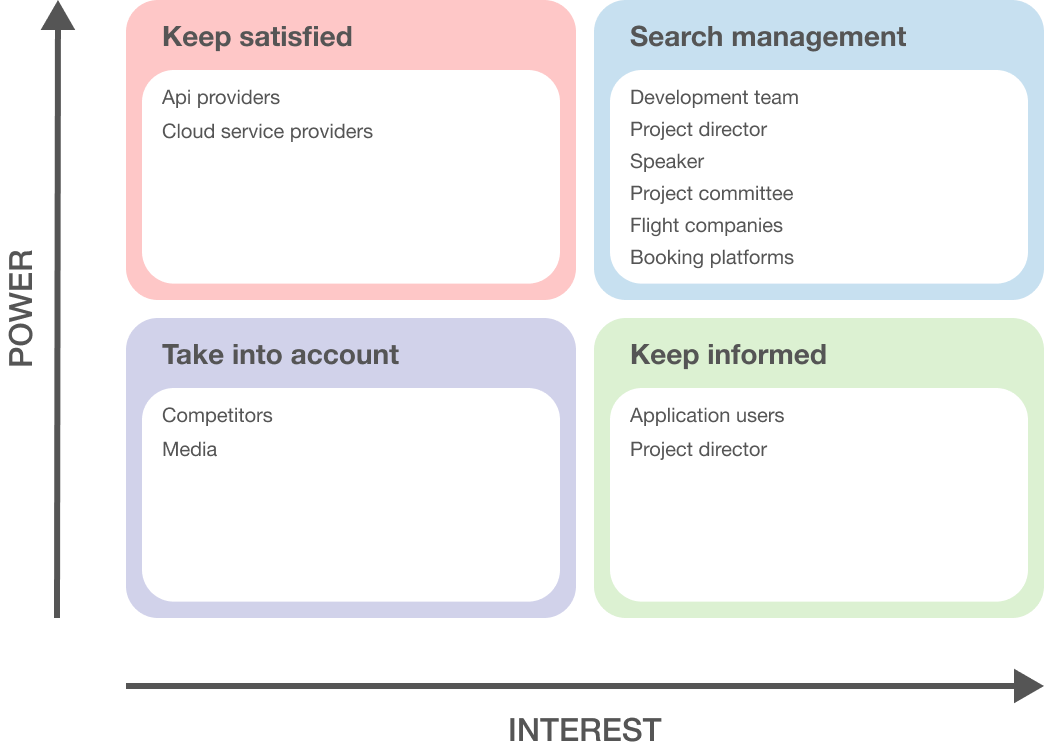
\includegraphics[width=\textwidth]{./assets/stakeholders.png}
	\caption{Representation of the stakeholders with the power-interest model}
\end{figure}
\begin{enumerate}[label = -]
	\item \textbf{Lower power and lower interest}
	      \begin{enumerate}[label = -]
		      \item \textbf{Competitors}: Other companies that provide equal or
		            similar solutions in the market.
		      \item \textbf{Media}: Media that is specialized in the same technology
		            and tourism.
	      \end{enumerate}
	\item \textbf{Lower power and high interest}
	      \begin{enumerate}[label = -]
		      \item \textbf{Final users}: Recurrent travelers that will habitually
		            use the application as well as taking advantage of the
		            notifications received.
		      \item \textbf{Families or recurrent travel companies}: Peopl that
		            could be indirectly beneficied from the application as it
		            simplifies the fact of keeping a connection with their
		            relatives, or those who can optimize their business model.
	      \end{enumerate}
	\item \textbf{High power and lower interest}
	      \begin{enumerate}[label = -]
		      \item \textbf{API providers and external services}: Companies that
		            will provide with the API servers and services that will be used
		            in the application development, yet they are not directly
		            involved with the project.
	      \end{enumerate}
	\item \textbf{High power and high interest}
	      \begin{enumerate}[label = -]
		      \item \textbf{Developers}: The team of 4 developers that will work in
		            the design, implementation and deployment of the application.
		      \item \textbf{Responsable de proyecto}: The person responsible for
		            supervising the project and providing guidance to the
		            development team.
		      \item \textbf{Speaker}: The project's Master's thesis evaluator, who
		            assesses the performance of the development team and the final
		            outcome of the project.
		      \item \textbf{Project committee}: La Salle URL faculty members who
		            supervise and evaluate the Master's thesis project.
		      \item \textbf{Airlines}: Air transportation companis that could
		            benefit from the market release of the application, due to the
		            utilization of air travel services by the app users.
		      \item \textbf{Booking platforms}: Companies that could integrate the
		            application into their services or that the application itself
		            could integrate into their search systems to enhance the
		            experience of their recurring customers.
	      \end{enumerate}
\end{enumerate}
\section{Alternatives analysis}
In the current landscape, there are other applications and travel-tech companies
that aim to address the needs of frequent travelers and optimize the habitual
joruneys. The following analysis overviews market alternatives, highlighting
their key features and potential differences with the Recurrent travel
application:
\begin{enumerate}[label = -]
	\item \textbf{TravelPerk}\cite{travel-perk}: TravelPerk is a business travel
	      management platform that offers a solution to plan, book and manage
	      corporate travels. The platform allows companies to centralise the
	      management of employee trips, establishin travel policies, optimize expenses
	      and enhance the traveler's experience. While TravelPerk focuses on the
	      corporate realm and is not specifically designed for recurrent travelers,
	      its cost optimization and travel management offerings could be considered
	      comparable to the ones offered by Recurrent travel.
	\item \textbf{Hopper}\cite{hopper}: Hopper is an applicatin that uses machine
	      learning algorithms to automatically predict and analise the tendencies of
	      flights and hotels, with the goal of helping users find the best offers.
	      Although Hopper is not focused in recurrent travelers, its focus to price
	      prediction and travel opportunity search could attract users of the
	      Recurrent travel. However, unlike Recurrent travel, Hopper does not allow
	      the possibility to configure customised trips taking into account user
	      preferences of time schedule, frequency and route.
	\item \textbf{Skyscanner}\cite{skyscanner}: Skyscanner is a flight, hotel
	      and car renting search engine, which compares prices between the
	      different service providers. Even though Skyscanner is a popular tool
	      to find travel offers, it is not specifically designed to attend the
	      necessities of recurrent travelers, as it does not provide the
	      configuration of time schedule, frequency and rote.
\end{enumerate}
To sum up, although there are several market alternatives in the travel-tech
sector, none of them specifically and comprehensively address the needs of
recurrent travelers in terms of presonalization, travel oportunity search and
cost optimization. Therefore, the proposal of Recurrent travel positions itself
as an innovative solution in the actual market, with the potential to
significantly enhance the experience of frequent travelers.
\section{Scope}
\subsection{Goals}
The master's thesis project Recurrent travel aims to develop a web application
that assists recurrent travelers in optimizing the planning and management of
their regular trips, offering a personalized and efficient solution for finding
the best travel deals based on their preferences. To achieve this objective, the
following sub-objectives have been identified:
\begin{enumerate}[label = -]
	\item Specific needs of recurrent travelers, particularly those who travel
	      frequently for work, family, or personal reasons, are identified and
	      analyzed.
	\item The current market of travel applications and services is investigated
	      to determine opportunities and gaps in relation to the needs of frequent
	      travelers.
	\item An easy-to-use web application is designed and developed, accessible
	      from various devices, allowing users to configure personalized trips by
	      specifying the route, preferred hours, ideal price, and travel frequency.
	\item Efficient search algorithms and techniques are implemented to find
	      relevant travel opportunities for users, utilizing Crawling/Scrapping
	      techniques and public APIs.
	\item A notification system is developed to timely and effectively inform
	      users about travel opportunities that match their preferences.
	\item The quality and maintainability of the developed software are ensured
	      by applying SOLID principles, Domain-Driven Design, hexagonal
	      architecture, and testing and validation techniques.
	\item The application is integrated with external systems and cloud
	      environments using continuous integration and deployment techniques to
	      increase software efficiency and ensure the rapid and constant delivery of
	      improvements.
	\item The application is integrated with different flight search platforms
	      like Skyscanner.
	\item The security and privacy of user data, including preferences, travel
	      history, and personal information, are guaranteed.
	\item The application is developed within an agile framework, focusing on
	      iterative and continuous value delivery, with defined delivery times to
	      ensure a timely response to business needs and adaptability to changes in
	      requirements.
\end{enumerate}
\subsection{Functional requirements}
The functional requirements describe the specific functionalities that the
Recurrent travel application must provide to meet its objectives and satisfy
user needs. The main functional requirements of the project are as follows:
\begin{enumerate}
	\item User authentication: The application must allow users to register and
	      authenticate to access their personal accounts and manage their
	      preferences and recurrent trips.
	\item Recurrent travel configuration: Users should be able to configure
	      recurrent trips by specifying the origin and destination, preferred dates,
	      and travel frequency.
	\item Flight opportunities search: The application must periodically
	      and automatically search for travel opportunities that match user
	      preferences, using Crawling/Scrapping techniques and/or public APIs.
	\item Filtering and result operations: The application must be able to
	      filter and sort search results for travel opportunities, considering the
	      corresponding user and the corresponding alert configuration.
	\item Flight opportunity notifications: The application must send
	      notifications to users when travel opportunities that match their
	      preferences are found, either by email or through messaging applications.
	\item Travel alerts management: Users should be able to manage received alerts by
	      marking them as read, archiving them, or deleting them, as well as modify
	      their notification preferences.
	\item Flight booking: Although it is not necessary for the application to
	      allow direct flight booking, it should facilitate the process by providing
	      links to airline websites or travel providers where users can complete the
	      reservation.
\end{enumerate}
\subsection{Non-functional requirements}
The non-functional requirements are those that describe the quality
characteristics of the system, such as usability, performance, security, and
scalability, among others. The main non-functional requirements of the
Recurrent travel project are as follows:
\begin{enumerate}
	\item Usability: The application must be easy to use and have an intuitive
	      and appealing interface, with a clear and consistent navigation structure
	      and presentation of information that facilitates user understanding and
	      decision-making.
	\item Performance: The application must be capable of performing travel
	      opportunity searches quickly and efficiently, offering results in a
	      reasonable time, even during high demand periods or with a large number of
	      concurrent users.
	\item Security: The application must protect users' personal information
	      and preferences by applying appropriate security measures, such as data
	      encryption, authentication and authorization, and prevention of common
	      attacks like SQL injection or cross-site scripting.
	\item Availability: The application must be available at all times,
	      ensuring high uptime and the ability to recover quickly from possible
	      failures or service interruptions.
	\item Scalability: The application must be able to scale to support the
	      growth in the number of users and resource demands, both in terms of
	      infrastructure and functionalities. This involves the ability to add new
	      servers, load balancing, and improving application performance as
	      necessary.
	\item Interoperability: The application must be able to interact and
	      integrate with external systems, such as airline APIs, using common
	      standards and protocols.
	\item maintainability: The application's source code must be easy to
	      understand, modify, and maintain, following established design principles
	      and patterns, such as hexagonal architecture, Domain-Driven Design, and
	      SOLID principles. Additionally, version control practices and adequate
	      documentation should be implemented to facilitate collaboration and
	      long-term project maintenance.
	\item Privacy and compliance: The application must comply with applicable
	      laws and regulations regarding the protection of personal data and user
	      privacy within the European framework.
\end{enumerate}
\subsection{Risks and barriers}
During the development process of the Recurrent travel project, several
challenges and barriers may arise that, if not taken into account, could result
in project failure or hinder its success. The following is an analysis of the
main challenges and barriers that may be faced:
\begin{enumerate}
	\item Changes in project requirements: Changes in project requirements may
	      occur throughout the application development, whether they are functional
	      or non-functional, requiring adjustments in the design and implementation.
	      These modifications could delay project progress and increase its
	      complexity and associated costs. To address this risk, it is essential to
	      properly plan and prioritize requirements, maintain constant communication
	      with stakeholders, and be flexible in adapting to changes.
	\item External applications integrations: The Recurrent travel application
	      will heavily depend on integration with external APIs and services from
	      airlines and travel providers. Access to these systems may be limited,
	      unstable, or change without prior notice, which would affect the
	      application's functionality and create issues in obtaining up-to-date and
	      accurate information. To mitigate this risk, it is crucial to establish
	      recovery mechanisms in case of failures, perform frequent integration
	      testing, and consider the possibility of using multiple data sources to
	      ensure information availability.
	\item Scalability and performance problems: If the application experiences a
	      rapid increase in the number of users and resource demands, scalability
	      and performance issues may arise, negatively impacting the user
	      experience. To address this risk, it is critical to design and implement a
	      scalable architecture, using appropriate techniques and technologies such
	      as cloud computing and load balancing, that allow adaptation to the
	      changing project needs.
	\item Privacy and compliance: The Recurrent travel application must comply
	      with applicable laws and regulations regarding the protection of personal
	      data and user privacy, which may pose challenges in implementing security
	      measures and respecting users' rights. To tackle this risk, it is
	      essential to stay informed about applicable regulations and incorporate
	      privacy practices from the design stage, ensuring that the application
	      meets legal requirements and safeguards user information.
	\item Time and resource limitations: The master's project has a limited time
	      for completion and may face constraints in terms of available resources,
	      such as the development team's time and allocated budget. These
	      limitations could affect the ability to successfully complete the project
	      within the established timeframe. To address this risk, it is crucial to
	      conduct proper planning, set realistic goals, and prioritize tasks based
	      on their importance and urgency.
	\item Market compeitition: The travel and transportation applications market
	      is highly competitive, with numerous players offering similar solutions.
	      This could make it challenging to differentiate "Recurrent Travel" and
	      position it in the market. To tackle this risk, it is essential to
	      identify and communicate the application's competitive advantages, such as
	      its focus on frequent travelers. Additionally, staying informed about
	      market trends and advancements, as well as being willing to adapt and
	      continuously improve the application based on user needs, is crucial.
\end{enumerate}
\section{Working methodology}
In further sections, the working methodology is explained in more depth.
Nonetheless, from the early beginning, the team decided to divide the work in
responsibilities. This division has allowed the team members, each with
different areas of expertise, be able to provide the project with their
knowledge in such areas.
\\
There have been bi-weekly meetings, with the goal to share to the team and the
team tutor what has been done during the last two weeks, as well as planning
what should be done the following. Furthermore, each meeting was an opportunity
to discuss with the tutor some of the project features and functionalities.
\\[8pt]
In terms of development, th team has organized through the GitHub Projects tool.
With this tool, it has been able to plan the tasks in a style that combines
elements of Scrum and Kanban. Being integrated with GitHub, it allows for a
seamless interactions between repositories and the project. For example, it
provides automation for moving tasks from one column to another.
\\
Since the team has worked mostly asynchronously, the usage of the board has been
crucial to give a view of the project status, as well as identifying what
elements were taking too much time, that were blockers of other tasks.
\begin{figure}[H]
	\centering
	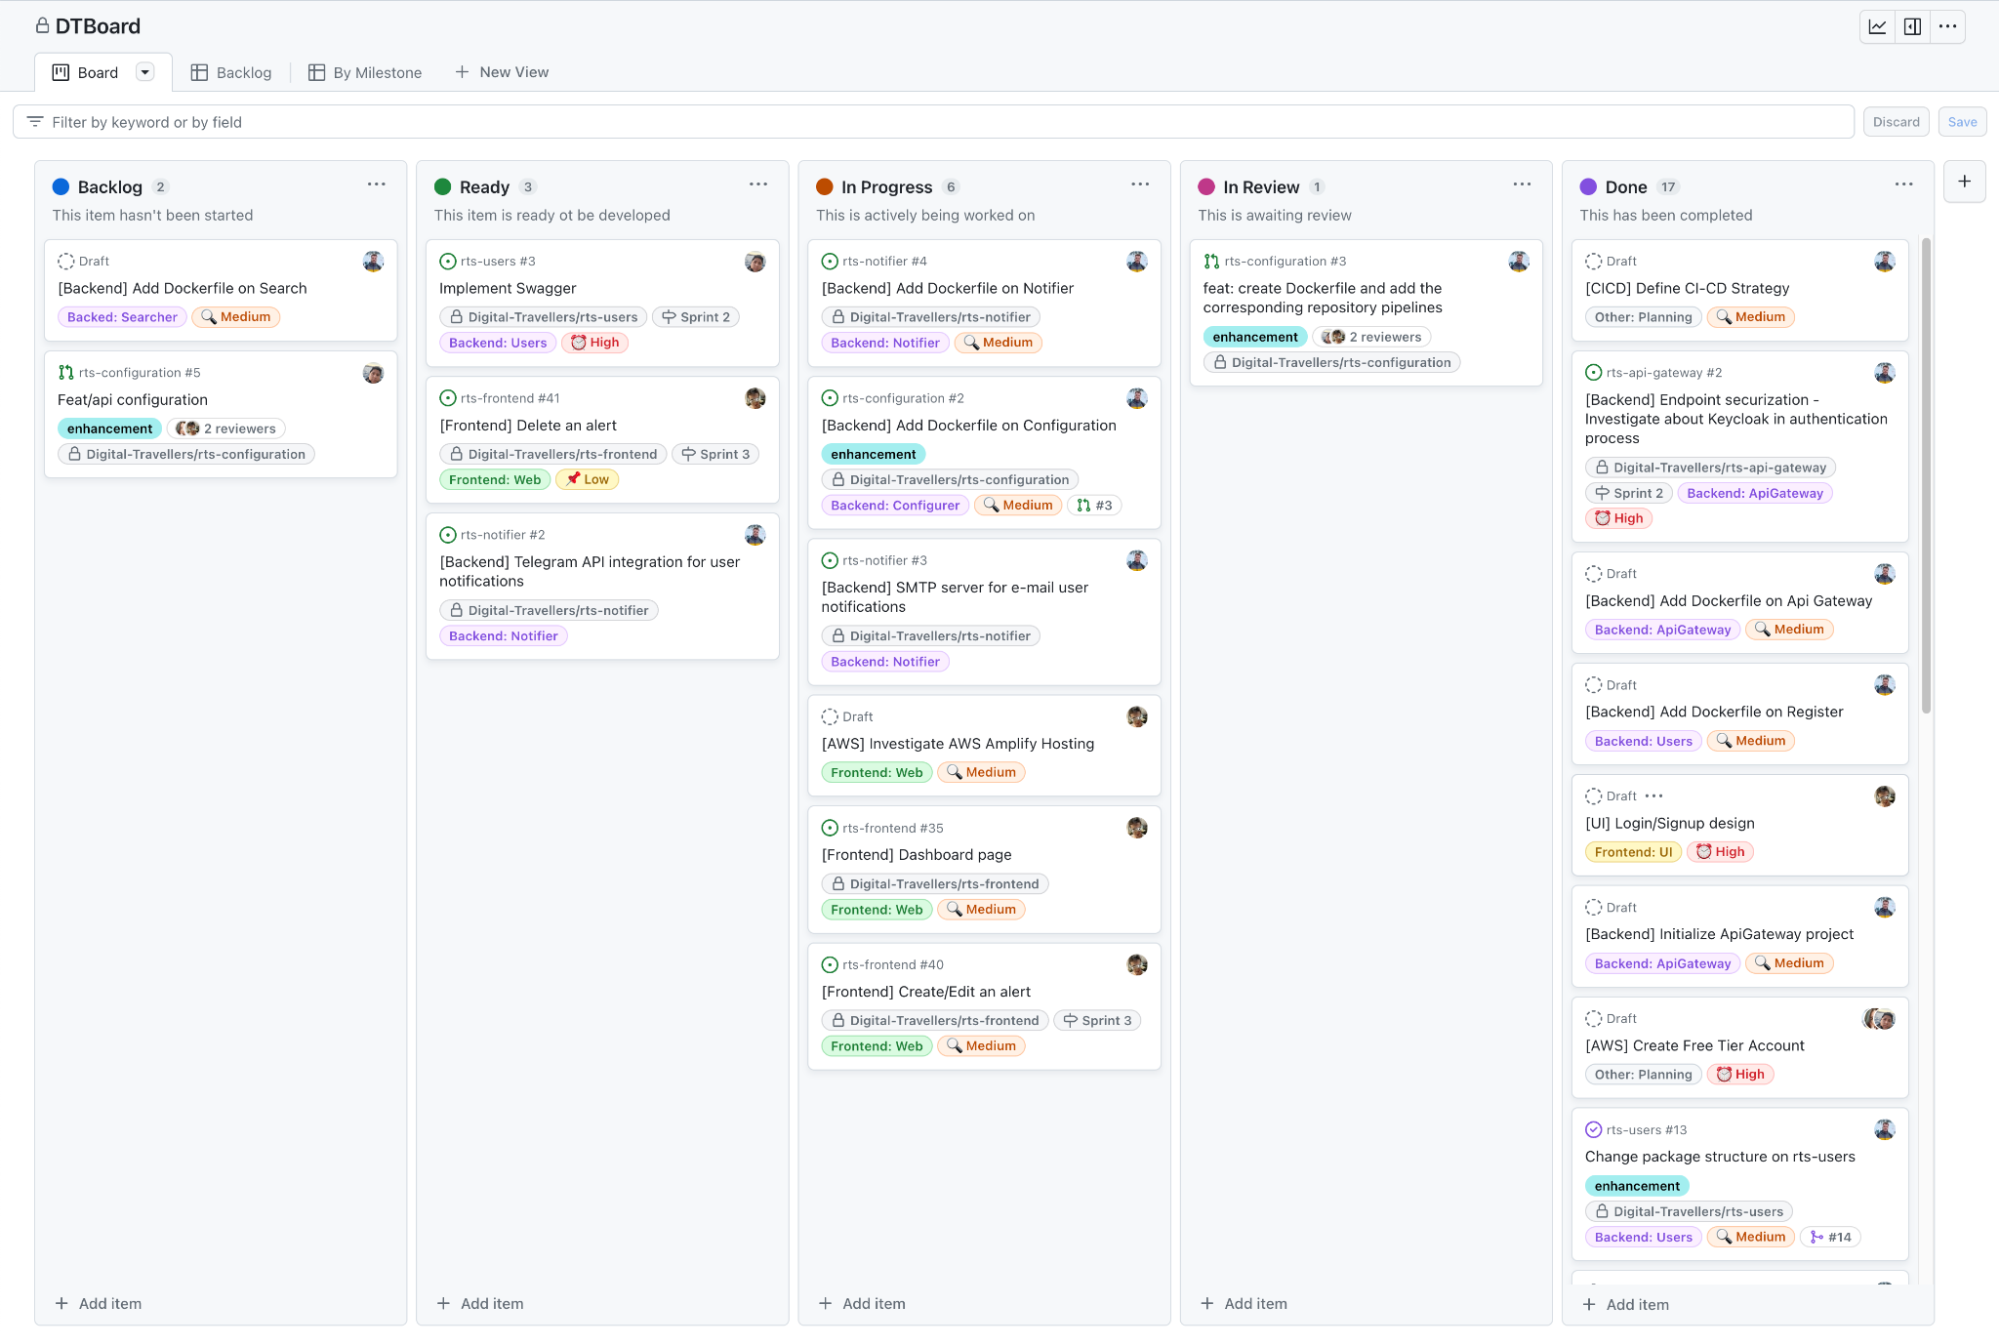
\includegraphics[width=\textwidth]{./assets/github-projects.png}
	\caption{Screen capture of the GitHub Projects tool}
\end{figure}
\end{document}
